\chapter{De la teoría a la práctica}\label{chap:B1}
\epigraphhead[50]{\epigraph{Es muy misteriosa, llena de figuras y cifras, oscura y no patente para todos. Tienen sus vocablos y maneras de hablar muy diferente significación de la que saben los vulgares trilingües. Por donde el que construyera la letra y tomare el sentido que resulta de la construcción gramatical caerá en muchos errores.}{Juan Huarte de San Juan, \textit{Examen de ingenios para las ciencias}}}
\section{Computador y papel}
Bien pertrechados de fundamentos teóricos sobre los que sostener el análisis de los textos, podemos por fin abordarlos empíricamente con garantías. En esta segunda parte formalizaremos lo visto hasta ahora para instruir al computador sobre el modo de aplicarlo a los textos y extraer de ellos la información requerida. ¿De qué manera lo haremos? Como adelantamos en la introducción, la idea es ir tomando lo expuesto en la parte que acabamos de concluir y formalizarlo en esta parte práctica empleando una notación algorítmica de \textit{pseudocódigo}\footnote{Llamamos \textit{pseudocódigo}\index{pseudocódigo} o lenguaje de descripción algorítmica a una representación informal compacta del paradigma de un algoritmo. Su función no es ser interpretado por una máquina, sino mostrar el principio operativo del algoritmo.}. En cierto modo, lo que ofrecen estas páginas no va a dejar de seguir siendo un desarrollo teórico, pues no usaremos código fuente \textit{real} de un lenguaje de programación específico que pueda ser copiado y ejecutado directamente en un computador, sino que encontraremos la idealización de formalizaciones generales. Estas idealizaciones se representan mediante una tecnología que ha probado su valía durante milenios: la escritura. Si bien intentaremos descomponer cada proceso en bloques relativamente sencillos para que puedan ser seguidos sin dificultad, un papel y un bolígrafo podrían ser de ayuda para orientarse en los pasos menos evidentes. 

Son tres las razones que nos animan a plantear la labor de esta manera y no comentando los listados de código del lenguaje de programación en el que hemos hecho las pruebas. En primer lugar, conviene proponer una idea de la forma más clara y concisa posible, por lo que haremos bien en abstraernos de las particularidades a las que están sujetos los lenguajes de programación. Estos obligan a emplear una sintaxis estricta y funciones muy específicas propias de cada uno de ellos, lo que exige descomponer las ideas abstractas en procesos menores concretos, más por satisfacer necesidades técnicas que conceptuales. Esto es, deberíamos atenernos a la literalidad de la computación de según unas reglas particulares y renunciar a los atajos contextuales que confieren al lenguaje natural su agilidad. Incluso cuando hay una traducción estructural biunívoca, existen diferencias en cómo expresar el desarrollo que requeriría aclaraciones. No solo serían así mucho más largos los listados —lo que sería un inconveniente menor—, sino también más farragosos y, por lo tanto, difíciles de seguir, lo que ya sí es una preocupación de primer orden.

En segundo lugar, cada lenguaje posee de un repertorio propio de expresiones internas con las que ejecutar operaciones sintéticas. Sin embargo, obligaría a hacerlo analíticamente allá donde no. Aunque todos los lenguajes suelen ser capaces de realizar operaciones elementales, la disponibilidad de recursos para abordar otras más complejas varía de un lenguaje a otro. Estas últimas —como, por ejemplo, aquellas relacionadas con el \ac{pln}— requieren \textit{bibliotecas}\footnote{Un \textit{biblioteca}\index{biblioteca} (\textit{library} en inglés, por lo que, con más frecuencia de la deseable, hay que leer traducido con el barbarismo \textit{librería}) es una colección externa de funciones que un programa importa para usarlas como propias.} externas en el mejor de los casos; en el peor, obligan a elaborar los procedimientos desde cero. Sea como fuere, aunque estas bibliotecas actúan como una caja negra cuyo mecanismo interno es ajeno al programa que las invoca, los datos de entrada, que hay que facilitarles, y los de salida, que devuelven, pueden variar significativamente en su formato, incluso cuando son conceptualmente equivalentes. Esta diferencia en el repertorio de los diferentes lenguajes hace que, como decimos, recurrir a uno en concreto ilustraría el uso particular en este, pero complicaría la traducción a otros. De ahí que el pseudocódigo sea una buena alternativa tanto por una cuestión didáctica como por su generalidad.

En tercer lugar, en relación con lo anterior, la explicación en un lenguaje de programación concreto ha de presuponer cierta familiaridad con algunos elementos sintácticos fundamentales que, de lo contrario, requerirían ser explicados. Dado que este no es el sitio apropiado para ello, una sistematización sin otras particularidades que las propias de una notación general facilitan la comprensión, si bien a cambio de llenar los huecos que deja la falta de un lenguaje de programación real con el sentido común del lector.

Sin embargo, no debemos olvidar que el objeto de este trabajo es práctico, queremos dar una solución a un problema real y, no solo eso,  la solución debe ser empírica. Por esa razón, no  dejaremos lo aquí expuesto en el mundo inteligible, sino que produciremos su realización sensible. Dicho de otro modo, no ha de preocuparse el lector, pues le ahorraremos el trabajo de traducir los algoritmos aquí presentados en programas informáticos: para poner a prueba lo discutido programamos una implementación completa en Python 3\index{Python}, la misma que, una vez depurada, se ha estado usando en el proyecto \textit{Sound and Meaning}, cuya última versión disponible a fecha de la entrega de este trabajo se encuentra en los apéndices o, en un formato más conveniente y en su última versión disponible, en los repositorios públicos que se han habilitado en Internet para ello.

Como ya habíamos adelantado, la ubicación de este capítulo antecediendo a la formalización de los aspectos teóricos no responde a la casualidad. Al contrario, se trata de una elección que —creemos— ayuda a comprender el resto del trabajo. En ese sentido, este capítulo es un puente entre los textos y programas reales y la idealización de estos que usaremos en los capítulos siguientes. Aquí se explica  la elección de bibliotecas externas y otras diseñadas \textit{ad hoc} en las que delegarlas, así como sus interrelaciones. Esto no es obvio y solo cobra sentido si se conoce de antemano la estructura de dependencia de los módulos en la implementación del modelo. Asimismo, tras el presente capítulo, asumiremos textos en condiciones ideales y no está de más conocer que llegar a ellos no es una cuestión trivial. Excúsese, pues, este interludio técnico.

\section{Modelo de pruebas}
Como hemos dicho, en esta segunda parte no encontraremos el prototipo final. En su lugar, trazaremos un plano en los siguientes capítulos para explicar qué ha de hacerse, aunque sin entrar más de lo estrictamente necesario en cómo ha de llevarse a cabo. Hallaremos, por ejemplo, \textit{listas}, pero no una forma concreta de añadirles nuevos elementos o recorrerlas, ya que esto entraría en las particularidades de cada lenguaje de programación: damos por hecho que el lector es capaz de componer mentalmente una lista y recorrerla de la manera que considere oportuno. Permanecemos, pues, en el ámbito de las ideas. Este capítulo contiene asimismo el conjunto de especificaciones técnicas del prototipo que pretendemos construir a partir de las instrucciones del «plano». El producto final, el resultado de aplicar todo esto —más bien su fotografía, como captura inerte del modelo real— es lo que encontramos en los apéndices.

\subsection{Lenguaje de programación}
Para realizar la implementación del modelo, podríamos haber empleado cualquiera de los muchos lenguajes de programación disponibles en el mercado, pues no faltan aquellos con capacidad para representar con sencillez las estructuras de datos y algoritmos que requerimos. No obstante, nos decidimos por la versión 3 de Python\index{Python} por varias razones que pasamos a detallar.

Nos hacemos una idea de las cualidades de este lenguaje de programación a partir de su definición como «\textit{general-purpose programming language that blends procedural, functional, and object-oriented paradigms}» \parencite[p. 6, énfasis en el original]{lutz2013}. Esto es, tenemos un lenguaje que permite abordar todo tipo de tareas y aproximarse a ellas según diferentes paradigmas. Concretamente, la orientación a objetos de Python contempla la encapsulación y reutilización sin complicaciones \parencite[xiii]{bird2009}. En la última década, Python se ha convertido en uno de los lenguajes de programación más importantes para tratamiento de datos, \textit{machine learning}\index{machine learning@\textit{machine learning}} y desarrollo de \textit{software} tanto en la academia como en la industria \parencite[2]{mckinney2018}.

Python es, además, un \textit{lenguaje de programación interpretado}\index{lenguaje de programación interpretado}. Esto es, el código fuente no se traduce a valores binarios de máquina\footnote{En la jerga técnica se conoce este proceso como \textit{compilar}.} para producir objetos autónomos\footnote{Una vez \textit{enlazados}, estos objetos podrían ser programas ejecutables independientes. Este es el caso, por ejemplo, del lenguaje de programación C, cuya compilación produce código binario para la máquina objetivo, o Java, en cuyo caso, el código binario está destinado a una máquina virtual.}, sino que es ejecutado por un intérprete para correr el programa. Esto tiene aspectos positivos y negativos. Por una parte, el proceso de interpretación es mucho más lento que la ejecución de código nativo. Además de la traducción a instrucciones de máquina, el código ejecutable suele estar más optimizado para la arquitectura física de la máquina. Sin embargo, compilar un programa requiere un tiempo considerable, por lo que tiene sentido en el caso de un programa pensado para ser distribuido como una versión definitiva, pero resulta inconveniente si se va a modificar el programa  constantemente, más aún si este no va a ejecutarse intensivamente más que un par de veces  frente a muchas de prueba. Esta es precisamente nuestra situación, por lo que el pequeño sacrificio en el tiempo de ejecución lo compensa con creces la agilidad que demuestra su despliegue, lo que en inglés se conoce como \textit{rapid turnaround}: favorece un desarrollo interactivo y ágil, probando en el momento, sin necesidad de recompilar el código fuente cada vez que se introduce una mínima modificación. No solo eso, sino que Python es además \textit{dinámico}, de manera que se asignan atributos y definen variables al vuelo \parencite[xiii]{bird2009}, al contrario que en los programas compilados de lenguajes clásicos, donde estos han de ser definidos por anticipado.

Otra de las ventajas de Python es su portabilidad. El mismo código se ejecuta en distintas máquinas con distintos sistemas operativos. El único requisito es que dispongan de un intérprete de Python. Este, por su parte, se puede descargar libre y gratuitamente. En nuestro caso, debía correr en todos los computadores de los miembros del proyecto \textit{Sound and Meaning} (Linux\index{Linux}, MacOS\index{MacOS} y Windows\index{Windows}), por lo que un lenguaje compilado hubiera planteado dificultades técnicas de cierta envergadura para portar los programas a máquinas con \textit{hardware} y un sistema operativo distinto al PC de tipo Unix\index{Unix} con el que se ha llevado a cabo el desarrollo \parencite[16-17]{lutz2013}. 

A pesar de esta flexibilidad, Python es un lenguaje de programación poderoso, dotado de recursos para llevar a cabo todo tipo de trabajos, incluso bajo la demanda computacional más exigente. Facilita la construcción modular de grandes programas y provee estructuras de datos predefinidas para ejecutar directamente operaciones relativamente complejas, pues estas están dotadas de herramientas para operar sobre ellas. Si las estructuras de datos básicas no satisfacen la demanda, las bibliotecas que incluye de serie expanden las facultades del lenguaje de programación mucho más allá de su funcionalidad básica. Y, como hemos dicho, a esto hay que sumar las bibliotecas de libre distribución de terceros \parencite[17-18]{lutz2013}.

A pesar de toda esta finura técnica, Python es fácil tanto de usar como de aprender, gracias a la transparencia de su semántica y sintaxis \parencite[xiii]{bird2009}. Incluso comparado con lenguajes de programación de alto nivel diseñados específicamente para fines didácticos, como Modula-2 \index{Modula-2}, Python resulta ganador en cuanto a sencillez de uso y legibilidad. Esto es así hasta el punto de que incluso ha llegado a denominarse \textit{pseudocódigo}\index{pseudocódigo} ejecutable \parencite[20]{lutz2013}. El lenguaje tiene fama asimismo de poder aprenderse rápidamente, aun sin experiencia previa en la programación, mucho más si ya se posee alguna con otros lenguajes.

Python es además libre y de código abierto. Esto no solo significa que su uso es gratuito, sino que se encuentra bajo una licencia que obliga a proporcionar el código y permite su redistribución sin restricciones, con independencia del grupo destinatario o los fines para los que se vaya a emplear, incluso para la creación de obras derivadas, que pueden ser redistribuidas en los mismos términos. La licencia compromete a preservar la integridad de la obra original en la distribución, pero puede ir acompañada de \textit{parches} para ser aplicados \textit{a posteriori}. Cualquier usuario al que le llegue el programa está sujeto a estas condiciones, que no cambian si el programa se distribuye como parte de otro y, recíprocamente, tampoco afectan a otros programas que se distribuyan junto a él \parencite{osi2007}.

No nos proponemos alterar el código de Python; ya hace lo que necesitamos muy bien. Por lo tanto, solo aprovecharíamos directamente de su carácter libre la posibilidad de usarlo sin costes adicionales. Sin embargo, esto presenta varias ventajas indirectas que nos afectan sobremanera. El movimiento del \textit{código abierto}  surgió en el seno de la comunidad del \textit{software libre}\index{software libre}, este último gestado en un ambiente académico  como una adaptación de los usos de ese entorno.
\blockquote{\begin{english}In a math department, anyone would be free to tinker with a proof that someone offered. If you thought you had a better way to prove a theorem, you can take what someone else did and change it. In a classics department, if you believed a colleague's translation of a recently discovered text was flawed, you were free to improve it. Thus, to Stallman, it seemed obvious that you should be free to tinker with and improve the code that ran a machine.\end{english} \parencite[279]{lessig2004}}
En palabras del ideólogo histórico del software libre Richard M. Stallman~\parencite*[57-62]{stallman2002}, el código abierto es una concesión pragmática que pasa por la renuncia al compromiso ético del movimiento original, para el que el software cerrado no es solo un inconveniente práctico, sino un problema social. No obstante, el uso de programas de código abierto supone un apoyo al software libre en la medida que ofrece una alternativa moralmente válida al código cerrado. En otras palabras, usando programas de código abierto, promovemos el libre intercambio de ideas y el acceso universal al conocimiento.

Sin renunciar a ese compromiso, lo cierto es que las ventajas pragmáticas del código abierto —si bien sus causas están íntimamente entretejidas con la naturaleza libre del software— no son desdeñables. En el caso de Python, esto se traduce en una enorme comunidad de usuarios y desarrolladores entusiastas. De esta manera, hay disponible una vasta cantidad de documentación que cubre la mayor parte de los problemas técnicos que uno se encuentra. Por otro lado, los miles de bibliotecas disponibles, tanto para llevar a cabo tareas generales como especializadas, alivian el desarrollo de los programas, pues evitan tener que reinventar la rueda una y otra vez en cada ocasión que a alguien quiere echarse a rodar\footnote{Existen bibliotecas de \ac{pln} como Stanza \parencite{qi2020} o SpaCy \parencite{explosion2023} con modelos avanzados para la lengua española. Hay, además, repositorios públicos de paquetes abiertos a contribuciones de los usuarios, por lo que no solo resulta instalar los desarrollos ajenos, sino compartir los propios. Esta flexibilidad para el usuario novel está muy por delante de la del resto de lenguajes de programación. Como nota adicional, si bien no de índole técnica, pero también con cierto peso en la elección, cabe mencionar el hecho poco conocido de que el nombre Python es un guiño al grupo de humoristas británicos Monty Python \parencite[20-21]{lutz2013}.}.

\subsection{Excurso \Roman{excurso}: Equipo}\stepcounter{excurso}
Podríamos valernos del lenguaje de programación como una formalización abstracta de los algoritmos que queremos implementar, de manera que tendríamos un pseudocódigo algo inflexible, pero bien estructurado, completo y sin ambigüedades. No obstante, nuestro propósito es aplicarlo a la práctica, por lo que necesitamos un computador que corra el código. Por lo tanto, lo aquí expuesto debe ser realizable y, en consecuencia, los planteamientos teóricos deben permitir una realización física factible. Dado que esto constriñe en cierta medida lo  que haremos, es menester mencionar estas cortapisas.

Con un presupuesto limitado, se hace necesario encontrar un compromiso de mínimos. Resulta mucho más práctico disponer no solo de una máquina capaz de correr programas en Python, sino también de llevar a cabo otras tareas, que ofrezca un entorno de desarrollo potente y versátil. De las soluciones que encontramos, la que más se ajustaba a las necesidades de este trabajo era una \textit{distribución} de \ac{gnu}/Linux\index{Linux}, por varias razones que pasamos a enumerar. En primer lugar, ofrece de serie una plataforma global con convenientes herramientas para la manipulación de texto como \textit{sed}, \textit{awk} o \textit{grep}. Provee asimismo editores de texto avanzados. Estos, además, admiten extensiones de terceros para incrementar sus capacidades, lo que permite configurar un entorno de programación completo dentro del editor (\Cref{fig:vim}).

\begin{figure}[!ht]
	\centering\small
	\resizebox{\linewidth}{!}{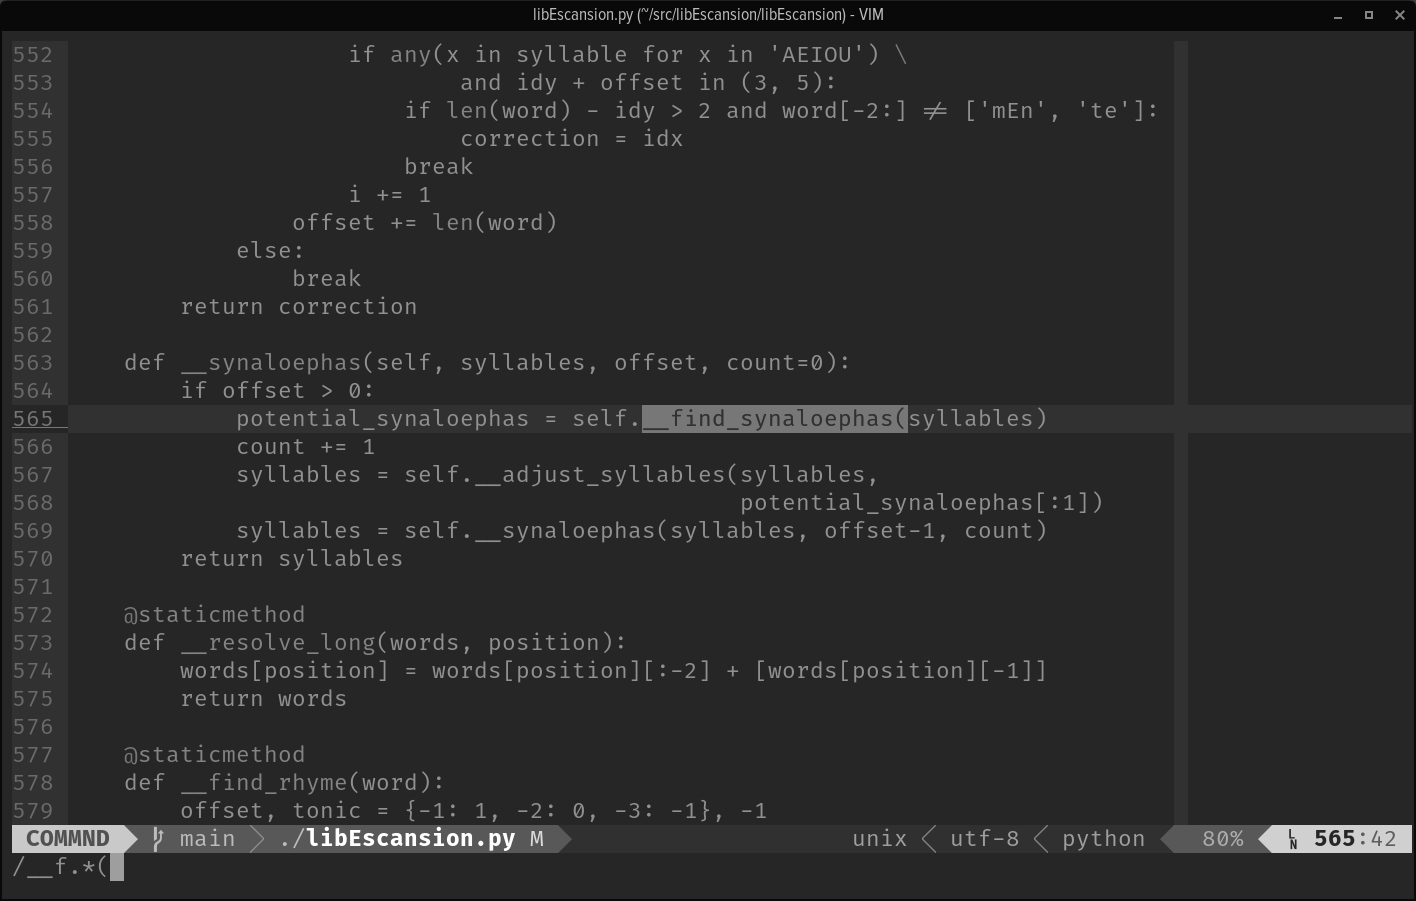
\includegraphics{images/vim.png}}
	\caption{Código Python en el editor de texto Vim.}
	\label{fig:vim}
\end{figure}

Otra cuestión a tener en cuenta es la filosofía \ac{gnu} y el software libre. Los paquetes empleados en el desarrollo de este trabajo son de código abierto y se encuentran bajo diferentes licencias libres. Esto garantiza el acceso a los programas y la libertad para usarlos sin restricciones ni coste alguno. Contra lo que podría suponerse, que los programas sean libres no compromete su calidad. Al contrario, se trata de estándares \textit{de facto} tanto en el entorno industrial como en el académico. Considérese, por ejemplo, el paquete de cálculo estadístico R\index{R} \parencite{r2019} o el propio Python en el ámbito del \textit{machine learning}\index{machine learning@\textit{machine learning}}: ambos son herramientas de uso mayoritario en su terreno.  El sistema operativo Linux, por su parte, ha demostrado su valía en aplicaciones científicas y comerciales hasta el punto de que los primeros quinientos supercomputadores más potentes del planeta operaban sobre alguna distribución de este sistema operativo\index{Linux} en noviembre de 2022 \parencite{top5002022} y domina el mercado de los servidores de internet \parencite{w3techs2023}. Creemos que nuestro trabajo, con unas exigencias mucho más modestas, bien puede aprovecharse también de estos recursos. No se trata, sin embargo, de una cuestión meramente práctica, sino que una porción sustancial del peso responde al compromiso ético con la libre difusión del conocimiento que encarna el software libre.

\begin{figure}[!ht]
	\centering\small
	\resizebox{\linewidth}{!}{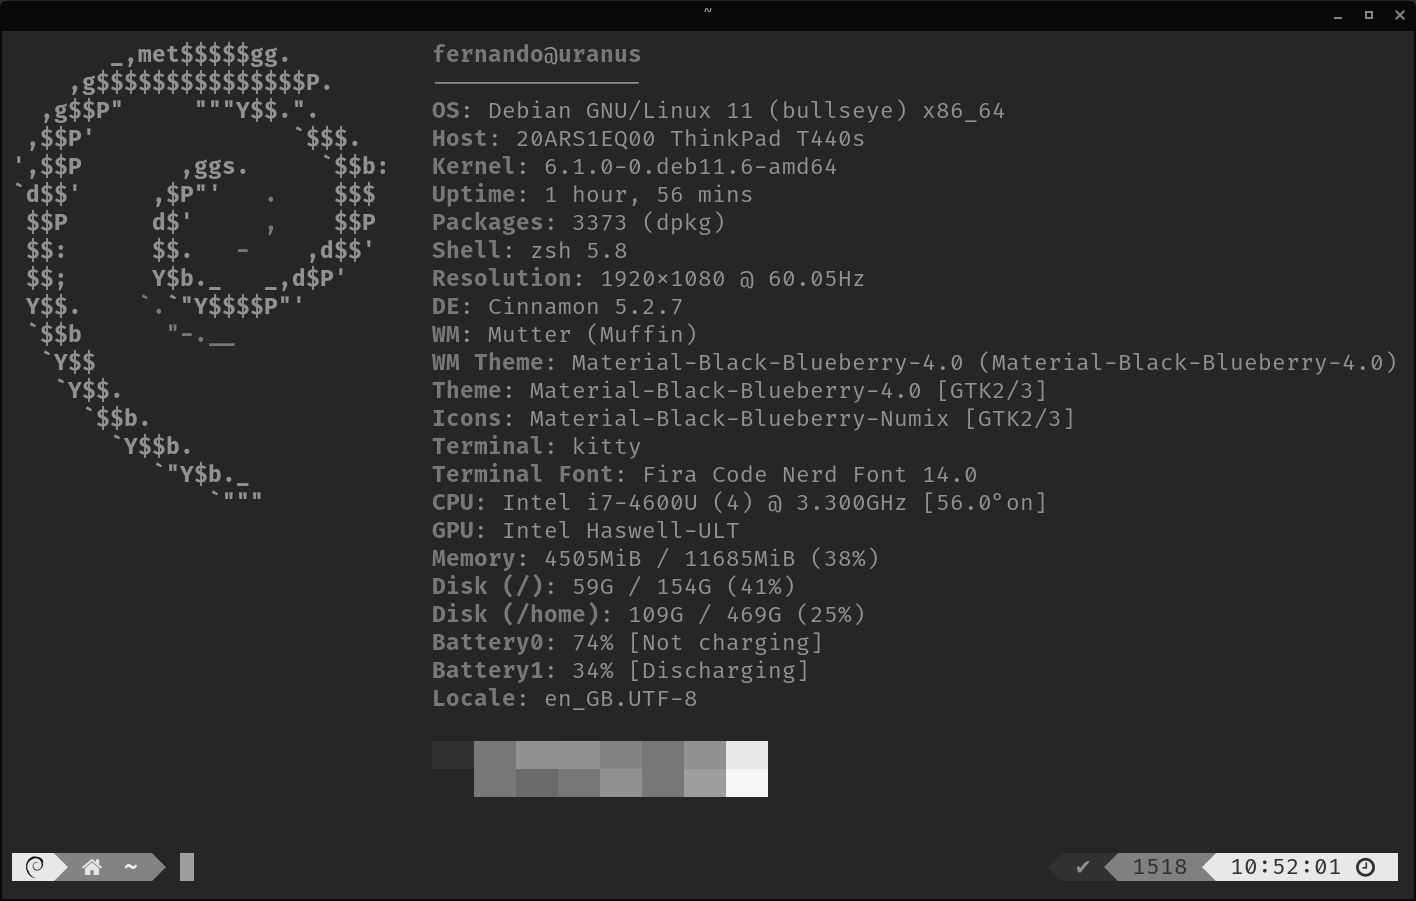
\includegraphics{images/neofetch.png}}
	\caption{Equipo de desarrollo.}
	\label{fig:neofetch}
\end{figure}

En concreto, optamos por la distribución Debian GNU/Linux\index{Linux} \parencite*{debian2022} en su versión 11 (\textit{Bullseye}), por aunar estabilidad con un completo catálogo de aplicaciones, a la vez que sigue una estricta política de licencias para seleccionar el software incluido. En cuanto al equipo físico, la mayor parte del trabajo se llevó a cabo en un Lenovo ThinkPad T440s con 12 GB de memoria RAM y un procesador de cuatro núcleos Intel CORE i7-4600U con una frecuencia de reloj de 3{,}3 GHz\footnote{Posteriormente, para procesar textos de manera masiva, encontramos que correr fragmentos del código en una GPU optimizada en lugar de la CPU del computador aceleraba sustancialmente los cálculos. Así, para la aplicación de los resultados del trabajo, empleamos los controladores comerciales de la empresa NVIDIA para poder ejecutar los programas en una tarjeta NVIDIA GeForce GTX 1060. De la misma manera, los programas completos se corrieron en diversas versiones del sistema operativo MacOS. En nuestro descargo alegaremos que, a pesar de que la portabilidad del programa deja correrlo en entornos más o menos cerrados, en su desarrollo nos ceñimos de manera estricta a software libre.} (\Cref{fig:neofetch}).


\section{Estructura del modelo}
Para plantear cómo construiremos el modelo, debemos conocer antes lo que va a hacer. En \Cref{fig:estructura} observamos una visión panorámica de los procesos que llevaremos a cabo, surgidos de depurar el concepto inicial \parencite{sanz2023a}. A grandes rasgos, tomamos los textos tal como los encontremos y los preparamos según su estructura dramática para obtener datos semiestructurados con los que el computador empiece a trabajar. No obstante, como analizaremos verso por verso, resulta más conveniente un formato que permita moverse en vertical de esta manera, por lo que tabulamos los datos y obtenemos uno estructurado. Estos datos son los que someteremos al análisis métrico, tal que la salida es una tabla con nuevas columnas para la información métrica de cada verso.

\begin{figure}[!ht]
	\centering
	\begin{tikzpicture}
	\node[datos] (input) {Datos no\\estructurados};
	\node[module, below=0.5cm of input](I1) {Preparación};
	\node[datos,right=1cm of I1] (semi) {Datos \\semiestructurados};
	\node[module, below=0.5cm of semi](I2) {Tabulación};
	\node[datos,right=1cm of I2] (est) {Datos \\estructurados};
	\node[module, below=0.5cm of est](I3) {Análisis \\métrico};
	\node[datos,right=1cm of I3] (output) {Texto \\procesado};
	
	\draw[->] (input)--(I1);
	\draw[->] (I1)--(semi);
	\draw[->] (semi)--(I2);
	\draw[->] (I2)--(est);
	\draw[->] (est)--(I3);
	\draw[->] (I3)--(output);
\end{tikzpicture}
	
	\caption{Estructura general.}
	\label{fig:estructura}
\end{figure}

En cuanto a la preparación, consta de una parte de limpieza semimanual variable, que consiste en convertir las fuentes en un formato legible para el programa y organizar el texto de acuerdo con su estructura dramática; esto lo veremos en detalle en el capítulo siguiente. En la primera parte habremos de recurrir en muchos casos a herramientas externas, mientras que la estructuración dramática se alcanza en gran medida mediante sustituciones con \textit{expresiones regulares}\footnote{Las \textit{expresiones regulares}  (abreviado \textit{\ac{regex}}, del inglés \textit{regular expression}) son una secuencia de caracteres con unas reglas sintácticas dadas que representan un patrón de búsqueda en un texto.}\index{expresión regular} una vez que el texto tiene un formato aceptable. Nos saltaremos este paso en ocasiones, siempre y cuando el texto a tratar esté ya semiestructurado, como es el caso de las ediciones en \ac{xmltei}. De cualquier forma, si los datos se hallan en un formato  adecuado, se convierten a datos estructurados de manera rápida sencilla mediante una herramienta para la manipulación automática de tablas.

Los datos tabulados resultantes son los que someteremos al análisis métrico.  Este se lleva cabo recorriendo la tabla por filas para escandir los versos uno a uno; la fila correspondiente se actualiza según los resultados con nuevas columnas.  El producto es una tabla de versos con anotaciones sobre las particularidades de cada uno en consonancia con su estructura métrica, función y jerarquía en la obra dramática.

\section{Módulos del programa}
Ya sabemos que Python cuenta con una inmensa cantidad de bibliotecas disponibles para llevar a cabo funciones comunes (y no tanto). Hemos de preguntarnos qué tareas podríamos delegar en ellas, si hay implementaciones capaces de encargarse de ello accesibles y, si es así, si estas satisfacen nuestras demandas. De lo contrario, no queda sino diseñar el procedimiento para resolver esas tareas desde cero. Como es natural, aceptaremos sin entrar en disquisiciones las bibliotecas que proveen fórmulas para llevar a cabo operaciones primitivas, esto es, aquellas que sirven para manipular tipos de datos básicos o interactuar con el sistema operativo. Nos centraremos, por el contrario, en las funciones abstractas tales como las representadas en la figura anterior. En nuestro modelo de pseudocódigo, al igual que hacemos en la implementación con el lenguaje de programación real, daremos por supuestas las funciones de tales bibliotecas y las emplearemos sintéticamente sin preocuparnos de su mecánica interna.

Por otra parte, no creamos programas para la limpieza y preparación de los datos, sino que trabajamos con herramientas preexistentes o sencillos \textit{scripts} para organizarlas, por lo que la configuración modular de los pasos más avanzados no afecta a esta etapa inicial. Los sistemas operativos de tipo Unix\index{Unix} están equipados de fábrica con potentes programas ya listos para hacer sin esfuerzo las operaciones que requerimos llevar a cabo. Los clásicos \texttt{sed} y \texttt{awk} para la manipulación de texto, por ejemplo, simplifican un tratamiento minucioso de los más pequeños detalles y admiten \ac{regex} para acotar las modificaciones. Otras herramientas facilitan los trabajos menos delicados, como convertir archivos de texto plano entre diferentes codificaciones. Incluso hay disponibles programas, como los editores de texto Vim y Emacs, capaces de hacer ambas cosas. Por lo tanto, este paso aconseja herramientas orientadas a un uso particular, más que recurrir a lenguajes de programación de uso general, sean reales, como Python, o ficticios, como nuestro pseudocódigo. Resulta mucho más sencillo resolver directamente las contingencias que surjan mediante pequeños mandatos de la línea de órdenes\index{línea de órdenes} provistos por el sistema operativo.

Una vez disponemos de los datos semiestructurados, empezaremos a automatizar realmente las tareas, ahora ya solventada la necesidad de supervisión humana. Para esto, por una parte, necesitaremos que el computador entienda el texto de entrada y, por otra, que conozca cómo estructurarlo en el formato de salida. Como veremos más adelante, tenemos previstos dos formatos semiestructurados: \ac{xmltei} y \ac{ved}, este último una notación simplificada propia para representar piezas dramáticas. Abordaremos cada uno de ellos de manera distinta. Para el primero, necesitaremos poder interpretar árboles \ac{xml} y, para el segundo, aplicar expresiones regulares\index{expresión regular} a las búsquedas. Sin embargo, entender la entrada, como decimos, es solo la mitad del trabajo. Hemos de ser también capaces de traducirla adecuadamente, por lo que necesitaremos algún tipo de herramienta que dé la posibilidad de trabajar con tablas. Las tablas, por su parte, son apenas el modo que tenemos de ordenar los versos. Una vez que hemos recorrido las líneas y llegado a la que deseamos, hay que extraer el verso de ella, escandirlo y modificar la línea mediante la adición de los valores correspondientes en nuevas columnas creadas al efecto.
 
De esta manera, si deseamos leer el texto semiestructurado, requeriremos herramientas para analizar jerarquías \ac{xml} y realizar búsquedas con expresiones regulares\index{expresión regular}. Tendremos que usar también algo que facilite la manipulación de tablas. Necesitamos, asimismo, algún instrumento para escandir versos. Para todas estas funciones existen diferentes bibliotecas disponibles listas para usar. La cuestión es: ¿debemos hacerlo? Empezaremos a responder la pregunta considerando las partes menos peliagudas.

El tratamiento de archivos \ac{xml}, la creación de un sistema de sustitución mediante expresiones regulares\index{expresión regular} y la manipulación de tablas son tareas que queremos completar, pero el modo de hacerlo es irrelevante para el propósito de este trabajo. Nos interesan los aspectos lingüísticos y literarios del análisis, no el mecanismo interno de las herramientas empleadas. Por otra parte, la escansión entra de lleno en las competencias de nuestra disciplina, así que nos ocuparemos de ella en detalle. En las pruebas de concepto, nos limitaremos a utilizar las bibliotecas estándar de Python para expresiones regulares y \ac{xml} y, para las tablas, emplearemos Pandas, por ser esta tal vez la biblioteca más popular para este tipo de tareas y, por lo tanto, de la que resulta más sencillo encontrar ayuda y documentación en caso de que se requiera. En el trabajo, obviaremos esas particularidades y asumiremos simplemente que podemos trabajar con tablas y expresiones regulares, sin entrar en cómo hacerlo.

De las bibliotecas de escansión que vimos en la revisión bibliográfica, apenas media docena se encuentran libremente disponibles. Asimismo, estas están orientadas a poemas\index{poema}, que no solo son textos monométricos, sino que además no tienen en consideración algunas irregularidades de los textos dramáticos. Esto hace necesario diseñar una herramienta de escansión específica para nuestro tipo de texto. En \Cref{fig:modulos} se esquematiza cómo se ha de llevar a cabo la escansión. Vemos que, además del conjunto de versos de entrada, tiene como salida los mismos versos ya procesados; una forma y otra se encuentran separadas por el programa encargado de análisis métrico. Dentro de este, se va recorriendo la tabla por filas para analizar los versos uno a uno; la fila correspondiente se actualiza en función de los resultados del análisis con nuevas columnas. De esta manera, escandimos cada uno de los versos y, para ello, etiquetamos gramaticalmente sus palabras para distinguir entre tónicas y átonas y hacemos la transcripción fonológica de cada palabra para trabajar con idealizaciones de sonidos y no grafemas.

\begin{figure}[!ht]
	\centering
	\begin{tikzpicture}
% Place Silabeador
\node[module] (I1) {Transcripción};
\node[module,right=0.5cm of I1] (I2) {Etiquetado\\ gramatical};
% Inner box around Items 2-3

\path (I2.north)--node[above=2mm] (arc) {Escansión} (I1.north);


\node[fit= (arc) (I1) (I2), draw, inner sep=2mm,rounded corners] (fit1) {};

\node[dato, above=1cm of fit1] (verso) {Verso};
\node[module,above=0.5cm of {verso}] (detabula) {Separación\\por verso};

% Pandas
\node[module,below=0.5cm of {fit1}] (I4) {Tabulación};
%arrow between boxes
\draw[->] (detabula)--(verso);
\draw[->] (verso)--(fit1);

\draw[->] (detabula)--(verso);
\draw[->] (verso)--(fit1);

\draw[->] (fit1)--(I4);

%upper label
%\path (fit1.north east)--node[above=15mm] (arc) {} (I4.north west);


\node[datos,left=0.5cm of verso] (Estrofas) {División\\estrófica};
\node[fit=(fit1) (I4) (detabula) (Estrofas) (I4), ,rounded corners, dashed,draw, inner sep=2mm, label={Análisis métrico}] (Overview) {};


\node[datos,left=1cm of Estrofas] (Input) {Estructura\\dramática};

\node[datos, right=0.5cm of Overview] (Output) {Texto\\procesado};



\draw[->] (Estrofas.north)|-(detabula);
\draw[->] (Input.east)|-(Estrofas);
\draw[->] (Overview.east) -- (Output.west);

\end{tikzpicture}
	
	\caption{Módulos.}
	\label{fig:modulos}
\end{figure}

Cabría cuestionar la conveniencia de delegar la transcripción y el etiquetado gramatical en bibliotecas externas. En cuanto a lo primero, se trata de una tarea compleja que requeriría, como mínimo, invertir tanto tiempo en ella como el que hemos dedicado a esta tesis. Por otra parte, existen diferentes herramientas disponibles capaces de llevar a cabo el proceso con una gran precisión. Por lo tanto, parece sensato dar un paso atrás aquí y tomar lo que se nos ofrece. En concreto, hemos optado por Stanza NLP. Se trata de una \textit{caja de herramientas}\footnote{\textit{Toolkit} en el original.} para Python de código abierto capaz de procesar más de sesenta lenguas, que incluye, entre otras funciones, la tokenización, lematización, expansión de tokens de varias palabras, etiquetado gramatical y análisis sintáctico. Dicho de otro modo, todo cuanto necesitamos. Esto lo ofrecen otros analizadores, como spaCy, pero Stanza rinde los mejores resultados para el español \parencite{qi2020}. Asimismo, se trata de un proyecto de investigación académica muy activo, por lo que el repositorio está abierto a contribuciones mediante el reporte de errores, que se resuelven en cuestión de horas. En el pseudocódigo consideramos tan solo una función genérica de \ac{pln}, lo que, recalcamos, se puede traducir de muy diversas maneras  en un lenguaje de programación, de modo que Stanza NLP es solo una posible forma de entenderlo.

El caso de la transcripción difiere del anterior. Las distintas bibliotecas para la fonología del español que hemos evaluado presentan dos problemas que desaconsejan usarlas. Por una parte, hay una dificultad de naturaleza técnica. Las bibliotecas están preparadas para transcribir exclusivamente texto con ortografía normativa, esto es, únicamente admiten los diacríticos comunes del español. Por lo tanto, no completan su labor si encuentran caracteres ajenos a esta lengua o, incluso, signos diacríticos típicos del verso, como la crema sobre vocales distintas de \textit{u}. El segundo inconveniente es conceptual: la división silábica no considera las excepciones a los diptongos ortográficos. Mientras que el primer obstáculo sería relativamente sencillo de solucionar mediante la edición del código fuente —que si es abierto, lo contempla— o la sustitución durante la preparación de los textos, el segundo requeriría una reescritura a fondo de los programas. Considerando el tiempo que habría que invertir en poner parches, estimamos que salía más a cuenta escribirlo desde cero, tomando nuestros requerimientos particulares como punto de partida y no como extras añadidos \textit{a posteriori}. Por el mismo motivo, el módulo de división silábica lo construimos también desde cero para ajustarlo a las demandas específicas de este trabajo. Esto permite, entre otras cosas, trabajar directamente con símbolos del \ac{afi} en las palabras a tratar.

En la implementación práctica nos valimos de otras bibliotecas adicionales, si bien estas resultan aún más irrelevantes para las disquisiciones de esta tesis. Entre ellas, se incluyen las dedicadas a tareas auxiliares como dibujar barras de progreso o cronometrar el tiempo de ejecución de los programas. Al ser estos elementos de control y no tener una función en el desarrollo del programa, como decimos, obviaremos tanto su uso como los motivos que llevaron a su elección.

\section{Formatos de las fuentes bibliográficas}
Para hacer las pruebas con el modelo necesitamos, huelga decirlo, textos: en particular, textos digitalizados. Hemos de dejar a un lado las condiciones ideales y enfrentarnos a las penurias del mundo real, despegarnos del \textit{texto} como idea y aproximarnos a sus realizaciones visibles. En definitiva, describiremos aquí los tipos de texto y procedencia de aquellos de los que nos hemos valido para llevar la abstracción a lo concreto.

Hay que empezar por decir que no existe un repositorio unificado de textos ni un formato estandarizado para codificarlos. Al contrario, los textos están muy repartidos y cada fuente parece tener una estructura propia, aunque superficialmente podrían antojarse similares. Los fondos semiestructurados suponen una minoría, si bien su número aumenta constantemente. Ha de tenerse en cuenta que, por lo general, el interés de la crítica se concentra en el reducidísimo conjunto de autores del parnaso canónico y, de su producción, apenas se presta atención a unas pocas obras selectas. Esto no es menos cierto en el ámbito de las humanidades digitales\index{humanidades digitales}, por lo que la probabilidad de dar con una buena digitalización de una obra menor es ciertamente escasa.

Desde el punto de vista técnico —por lo menos en lo que concierne al texto, sin entrar en cuestiones de composición y tipografía—, la labor se reduce a media decena de tipos de archivos, varios de ellos tratables con las mismas herramientas. Tenemos datos semiestructurados en \ac{xmltei} y otros no estructurados de texto, como \ac{html} y texto plano, así como también otras codificaciones más complejas, como \ac{pdf}. Asimismo, encontramos formatos para procesador de texto, como \ac{doc}\footnote{Lamentablemente, los formatos de archivo comerciales predominan sobre los abiertos, lo que, más allá de nuestro trabajo, pone trabas al intercambio de información y conocimiento cualesquiera que sean los fines.}. 

El propósito de este trabajo es, además, equipar al proyecto Sound and Meaning con una herramienta capaz de extraer datos de obras teatrales áureas e incorporar los textos junto a sus metadatos a un corpus. Este está destinado a servir como fuente para la investigación, por lo que es prioritario que los resultados de estos sean válidos. Esto obliga a restringir las fuentes según una serie de criterios que lo garanticen. Así, para hacer pruebas solo hemos tenido en cuenta las ediciones con las que trabajaba el proyecto. No debe entenderse esto como una limitación técnica, pues, en teoría, el modelo podría analizar textos que no se atuvieran a estos criterios, a pesar de que únicamente aseguraría resultados adecuados cuando aquellos se observan.

Las posibles obras candidatas para el análisis se reducen si tomamos la precaución de considerar solamente aquellas que cuentan con ortografía normalizada y modernizada. Aunque hemos intentado que los modelos sean capaces de procesar la gran mayoría de las grafías que se encuentran en las digitalizaciones de obras teatrales auriseculares, con independencia de la edición, no debemos olvidar que asumimos criterios ortográficos y fonológicos modernos. De esta manera, los resultados producidos por un texto normalizado y otro sin normalizar podrían no ser comparables debido a la imprevisibilidad del último. Es más, es posible que este tenga inconsistencias internas, lo que podría invalidar incluso un examen individual. Por lo tanto, quien haya de servirse de nuestro trabajo debería tener esto en cuenta a la hora de seleccionar las fuentes que va a usar, pues la consistencia de los análisis con ortografías no normalizadas ofrece garantías insuficientes, máxime si las convenciones de partida divergen.

La escasez de textos es aún más cierta si lo que buscamos son buenas ediciones. Lamentablemente, no todas las fuentes que se encuentran digitalizadas responden a unos criterios mínimos de calidad ecdótica. Por lo general, no presentan problemas generalizados, pero unas pocas ediciones de origen oscuro muestran deficiencias graves, alguna de ellas capaces de alterar el valor de las distribuciones de los ritmos. Por este motivo, el proyecto Sound and Meaning solo ha trabajado con textos de prestigio, pues lo contrario habría obligado a llevar a cabo un minucioso examen filológico de cada edición de procedencia no fiable para verificar su calidad; ahora multiplíquese ese tiempo por los cientos de posibles candidatos. De esta manera, aunque es probable que se hayan excluido muchos textos perfectamente válidos por carecer del aval de un editor, lo cierto es que simplifica la composición del corpus, al permitir integrar nuevos textos de inmediato. Por consiguiente, si ha de incluirse un texto de procedencia incierta, conviene tomar la precaución de examinarlo bien antes de encomendarse a los resultados de su análisis para extraer conclusiones.

Sea como fuere, con estos mimbres hay que hacer el cesto, por lo que más vale acostumbrarse a ello. En una situación óptima, dijimos, encontramos datos semiestructurados, como en el caso del corpus calderoniano  \parencite{caldracor2022}, por ejemplo. Asimismo, las obras de Artelope \parencite{oleza2022} y  T\textsuperscript{\underline{c}}/12 \parencite{tc12}, aunque no se encuentran directamente accesibles en \ac{xmltei}, aparecen como datos estructurados incrustados en el código HTML de las páginas donde se presentan las obras. Por los notables paralelismos entre las estructuras, podría sospecharse incluso que la página web se ha generado automáticamente a partir de una edición en \ac{xmltei}. Sin embargo, si bien la situación ha mejorado notablemente en la última década, siguen estando tan vigentes como entonces los \textit{desiderata} de \citeauthor{valdes2014b}~\parencite*{valdes2014b}. 

La mayoría de las fuentes de donde partimos presentan sus textos en formato \ac{pdf}. Las principales Prolope~\parencite{prolope2023} para comedias de Lope de Vega y GRISO~\parencite*{griso2020}, que dispone de una completa colección de autos sacramentales de Calderón. Esta disponibilidad, junto a los textos de CalDraCor, hace que, a día de hoy, la obra calderoniana sea posiblemente la más apta de entre sus contemporáneas para llevar a cabo estudios digitales. No podemos dejar de mencionar la Biblioteca Virtual Miguel de Cervantes \parencite{cvc2021}, aunque, en este caso, dada la diversidad de las procedencias editoriales de sus fondos, conviene seleccionar las obras individualmente.

Finalmente, tenemos obras recopiladas individualmente gracias a la generosidad del propio editor. Estas suelen encontrarse en los formatos propios de los procesadores de texto que incluyen los paquetes ofimáticos comunes. Dado que, en este caso, los textos se obtienen normalmente de forma individual e, incluso un mismo editor se vale de diversas herramientas a lo largo del tiempo —téngase en consideración que el rango temporal de estas ediciones va desde principios de la década de 1990 a textos que acaban de terminarse y aún no están publicados\footnote{Prolope, Instituto de Teatro Clásico de Almagro,  comedias.org y CANON60, entre otras.}—, estas ediciones son tremendamente heterogéneas.  Dada esta variedad de procedencias, nos enfrentamos a diferentes obstáculos para preparar los textos de manera que podamos emplearlos directamente en el computador.

\section{Diferencias entre textos, textos y textos}
La heterogeneidad de los textos requiere aproximarse individualmente a los problemas que presenta cada uno de ellos. No solo nos hallamos ante una plétora de formatos incompatibles entre sí, sino que, incluso, encontramos diferencias en la manera en que se codifican dos textos en el mismo formato. La diferencia principal estriba en que algunos de esos formatos proveen facilidades para la manipulación y análisis textual; otros, por el contrario, suponen un obstáculo que, en ocasiones, resulta insalvable.

El primero de los retos que uno se encuentra para tratar un texto digitalizado —y no por obvio deja de ser el más importante— es obtener el susodicho texto. Aquí se distinguen varias tipologías: por una parte, los textos accesibles públicamente y, por otro, aquellos que no lo están y han de obtenerse a través de diversas vías, como el préstamo o la compra. Estos textos, con independencia de cómo se hayan conseguido, pueden ser libres o tener restricciones legales o técnicas. Esto es, hay textos que prohíben la manipulación y copia en cumplimiento de los derechos de autor, lo que se fuerza en ocasiones mediante la aplicación de un sistema de protección digital anticopia. No obstante, se encuentran textos de dominio público con la misma protección, lo que también impediría tratar un texto, aunque fuera perfectamente legítimo.

Asumiremos que trabajaremos legalmente con los textos de los que disponemos y que estos no están restringidos por protección digital alguna. Los formatos más comunes son \ac{pdf}, TXT, \ac{xml} y cualquiera de los tipos de archivos privados e incompatibles entre sí —incluso entre diferentes versiones de supuestamente el mismo programa— de los diversos procesadores de texto\footnote{En el curso de los trabajos llevados a cabo para el proyecto Sound and Meaning, pudo comprobarse que, lamentablemente, los archivos creados con un procesador de textos suelen estar en alguno de los diferentes formatos cerrados de Microsoft Office; excepcionalmente, aparece algún archivo en Open Document Format (\ac{odf}). Como anécdota, algunas de las obras del corpus del proyecto estaban compuestas con WordPerfect 5.2, una versión del programa salida al mercado en 1992; aunque los procesadores de texto comerciales modernos fueron incapaces de reconocer ese formato, el paquete ofimático libre LibreOffice.org no tuvo problema para abrirlo.}. Una vez se dispone de acceso al archivo, el objetivo es convertirlo a datos semiestructurados. En el caso de \ac{xml}, se obvia ese paso porque ya lo está.

\section{Peor escenario: PDF}
Los archivos \ac{pdf} albergan el texto completo, pero este no es directamente accesible. No se trata de un texto plano ni de un lenguaje de marcado como \ac{xml}, sino de una descripción de las páginas. Para poder verlo, requerimos de la mediación de un programa capaz de interpretar el código binario del archivo y representarlo de manera visual en la pantalla. Se presenta el problema de que, de esta forma, no hay posibilidad de trasladar la composición de la página directamente y, por lo tanto, tampoco la estructura de la obra. Se necesita convertir ese documento a texto plano y, a la vez, preservar el mayor número de elementos visuales posible, de manera que se minimice el trabajo manual. La forma de hacerlo dependerá de como se haya compuesto el archivo, ya que esto determina el modo en que se codifica el texto.

Cada una de las páginas contiene bloques de instrucciones que definen segmentos de contenidos y sus características. En el caso de los bloques de texto, estos suelen estar repartidos de acuerdo no a un criterio textual, sino a las necesidades de la maquetación. Por ejemplo, para representar \textit{Ejemplo}, ubicaría la \textit{E} en la posición $(x,y)$  y el segmento \textit{jemplo} en $(x+1-n, y)$, de modo que desplazaría el segundo segmento $n$ puntos hacia la izquierda para hacer un acoplamiento parecido a \textit{Ej}, en lugar de conservar el espaciado como en \textit{E\strut j} \parencite{glyph2022}. Esto hace que los programas para la extracción automática del texto aborden la tarea colocándolo en orden de lectura sin más. La complejidad de la maquetación y su proximidad a la jerarquía textual son determinantes para decidir la manera de abordar el texto.

Si la maquetación del documento se aviene hasta cierto punto a la estructura textual, recurriremos a herramientas de conversión de formato como \texttt{pdftotext}, que dan la opción de conservar la distribución espacial de  los elementos en la página, aunque no consigan un resultado perfecto.  Después, el trabajo consistiría en afinar esta conversión mediante expresiones regulares\index{expresión regular}. De esta forma,  se eliminan cabeceras de página, numeración de los versos múltiplo de cinco y aparato crítico, así como las voladas de llamada a nota si las hubiera. Esta parte no presenta muchas dificultades, ya que los saltos de página vienen marcados con un metacarácter.

Sabemos que la primera línea tras el salto de página es la cabecera, por lo que se elimina. Los números de verso aparecen a la derecha del texto, precediendo de manera inmediata al final de línea y después de uno o más espacios o tabuladores que los separan del texto. Sabiendo esto, suprimimos los guarismos que cumplan esas condiciones, ya que no encontraremos un equivalente textual. No suele haber llamadas a nota porque la numeración se corresponde con el número de verso. Si las hubiera, no obstante, esto tampoco presentaría excesivo problema, ya que las llamadas van anejas a una palabra o a un signo de puntuación no precedido por un guarismo y, en este último caso, seguidas de espacio. Aunque, hipotéticamente, podrían darse casos como \textit{123\textsuperscript{1}}, los guarismos intratextuales son prácticamente inexistentes, por lo que asumimos simplemente que varios de ellos a final de línea son cifras del mismo número.

Las notas a pie de página, sin embargo, admiten el tratamiento directo  con dificultad. Sabemos que entre las notas y el cuerpo textual hay varias líneas de espaciado, a semejanza de la composición del texto de origen. Desafortunadamente, esto no se da siempre ni todas las veces que lo hace indica la separación entre ambas entidades. Con la numeración de las notas sucede lo mismo: da una pista, pero no es ni necesaria ni suficiente. La segunda línea y subsiguientes de una nota de más de un renglón no van precedidas de un guarismo, como tampoco lo van la continuación en la siguiente página de una nota extensa. Por otra parte, cuando alternan varios personajes genéricos del mismo tipo, estos se nombran a veces simplemente mediante sus ordinales, como \textit{1.º}, \textit{2.º}, etc., por lo que, aparte de la numeración a principio de línea, se requieren otros criterios. Un tercer indicio es la longitud de la línea, si bien aquí también encontramos tanto parlamentos en prosa de líneas largas como notas tan cortas como un verso de arte menor. La combinación de estos criterios no es una garantía lógica de los aciertos, si bien, en la práctica, es suficiente. Así, buscaremos líneas largas antes del final de página que estén separadas por varios espacios del cuerpo principal y líneas largas que comiencen por un número y las siguientes hasta el final de la página.

El cuerpo del texto no es uniforme. Por una parte, las líneas\index{línea} y las didascalias de personaje\index{didascalia de personaje} suelen presentar pocas dificultades porque el sangrado revela la función y este se conserva al convertir entre formatos. Hay, empero, dos elementos textuales que requieren una inspección visual detenida: las acotaciones\footnote{Trataremos la didascalia de personaje como un elemento distinto al resto de acotaciones, pues estas tendrán entidad propia, mientras que aquella proporcionará un atributo.} y los versos compartidos. Las acotaciones\index{acotación}, salvo que vayan centradas en la página, no se distinguen de otros componentes textuales porque el texto plano no tiene la capacidad de aplicar formato a los caracteres. Por lo tanto, los fragmentos en cursiva del archivo \ac{pdf} de origen se traducirían en redonda en el de texto plano. Esto hace inevitable el marcado manual. Las continuaciones de versos compartidos, por su parte, se ven o no dependiendo de si el espaciado original es suficiente como para que la herramienta de conversión lo interprete como tal. Un espaciado insuficiente implica que en el archivo de texto no habrá distinción en el sangrado de un verso normal y la continuación de un verso compartido. Si bien suelen encontrarse fallos en la segunda parte del verso, a partir de la tercera, al llevar dos niveles de sangrado, resulta más infrecuente. En cualquier caso, conviene hacer un examen manual para marcar estos versos. El proceso consiste en un primer cotejo visual para buscar últimos versos de un parlamento y primeros del siguiente más cortos que los del bloque les rodea. Una vez localizados, se verifica que ambas líneas componen un solo verso y se ajusta el sangrado si procede.

Puede darse la situación de que un archivo  \ac{pdf} con una estructura interna compleja produzca unos resultados tan pobres s al convertirlo tratando de conservar la maquetación, que requiera tal cantidad de correcciones manuales que se dispare el tiempo necesario para preparar el texto. En algunos de estos casos, es posible usar una alternativa geométrica. Ahora emplearíamos otra herramienta para convertir a lenguaje de marcado, tal como \texttt{pdftohtml}, para traducir el archivo \ac{pdf} a \ac{xml}. El resultado no se trataría de un \ac{xml} como en la jerarquía definida por \ac{tei}, sino que los elementos se caracterizarán por su posición espacial. Estos poseen atributos que indican mediante pares de coordenadas su ubicación física en la página. Con esto en mente, estimamos los rangos en los que comienzan los elementos horizontalmente en cada página. Es importante porque, además de variar la maquetación en general entre páginas pares e impares, hay elementos que no aparecen en todas las páginas. Así, los fragmentos centrados incrementarían el rango, cuyo punto de inicio sería la mitad de cuerpo de texto para un solo carácter. Lo mismo sucede con las continuaciones de versos compartidos, cuya posición inicial depende de la longitud de la parte precedente del verso en la línea o líneas anteriores.  Por el desplazamiento vertical sabemos a qué línea corresponden los segmentos. Sea como fuere, ya es factible aproximar con cierta exactitud la distribución de los elementos y pasar el \ac{xml} a texto. A pesar de ser un método más engorroso que el anterior, presenta al menos una ventaja sobre aquel, en tanto que se conservan los atributos de los caracteres, con lo que se encuentran las acotaciones con más facilidad. No resulta esta tampoco una solución infalible porque, por ejemplo, una expresión latina intercalada a comienzo de verso sería indistinguible de una acotación interna como \textit{Canta} si esta última no va entre paréntesis.

La carga de temporal de este tipo de conversiones es variable, pero el coste por obra ($C$) es inversamente proporcional al número total de obras ($n$), en tanto que se requiere invertir una cantidad notable de tiempo ($T_0$) para establecer reglas que evalúen los patrones de la primera y aplicarlas a cada una de las siguientes ($i$) de manera mecánica, lo que toma una pequeña cantidad de tiempo ($t$) en comparación con el necesario para encontrarlas.  

\begin{equation}\label{eq:tiempo}
C = \frac{T_0 + \sum_{i=0}^{n} t_i}{n},\: t_i \ll T
\end{equation}

En términos llanos, esto es que, si disponemos de varios archivos con la misma estructura interna, solo tenemos que encontrar las reglas en uno de ellos y, una vez con ellas, podemos aplicarlas en bloque al resto de textos. Por lo tanto, cuantos más fuentes de la misma procedencia obren en nuestro poder, más eficiente en tiempo será convertir cada uno de ellas. Por el contrario, el peor escenario en términos de efectividad sería tratar una obra suelta. En el caso del corpus de \textit{Sound and Meaning}, casi un centenar de archivos PDF procedían de las digitalizaciones del GRISO \parencite*{griso2020} de autos calderonianos. Todos ellos respondían al mismo modelo y pudieron ser tratados mediante la conversión directa a texto plano. Esto hizo posible crear un corpus de varios cientos de obras a pesar de partir de \ac{pdf}.

\section{Escenario regular: archivos ofimáticos}
Con archivos ofimáticos nos referimos a aquellos formatos producidos por el programa de edición de textos de un paquete para trabajos de oficina, como Write de LibreOffice.org o Word de Microsoft. Nos encontramos con estos archivos sobre todo en casos en los que el propio editor de la obra se la ha facilitado al proyecto \textit{Sound and Meaning}. La manera de codificar el texto con formato varía sustancialmente; oscila entre estándares abiertos como \ac{odf}, que internamente usan archivos \ac{xml} comprimidos, y cerrados diseñados específicamente para mantener un mercado cautivo, como es el caso del formato \ac{doc} de Microsoft y su plétora de versiones y revisiones apenas parcialmente compatibles, incluso entre sí. En cualquier caso, una vez conseguimos abrirlos mediante el programa correspondiente, trabajaremos con ellos sin complicaciones, ya que no requerimos recurrir a las extensiones propias más esotéricas, sino simplemente algunas funciones elementales para manipular texto con formato. En concreto, tienen importancia la alineación del párrafo, las sangrías y algunas propiedades de los caracteres (cursiva y versalitas, sobre todo). El objetivo es convertir a texto plano marcando de alguna manera esas propiedades para poder conservarlas.

Los elementos que afectan al párrafo y la línea se marcan atendiendo  a su espaciado. No es así con las propiedades de los caracteres, ya que estos pueden ir intercalados entre otros sin formato adicional. De este modo, marcaremos estos con una etiqueta reconocible, esto es, una serie de caracteres que no se vayan a dar en el texto. Si bien esto añade artefactos al formato, reconocerlos y tratarlos como tales es trivial, por lo que las ventajas superan con creces los inconvenientes, que son de orden estético en cualquier caso. 

Para este trabajo, nos hemos servido del paquete LibreOffice.org porque da la posibilidad de buscar y reemplazar mediante la combinación de expresiones regulares\index{expresión regular} estandarizadas y elementos de formato, por lo que los pasos que lo requieren pueden darse fácilmente. La extensión \textit{Alternative Find \& Replace for Writer} hace posible otras sustituciones. Las alternativas existentes, como Microsoft Office, ofrecen herramientas con una funcionalidad restringida en comparación. Así pues, optamos por la alternativa libre.

\begin{figure}[!ht]
	\centering\small
	\resizebox{\linewidth}{!}{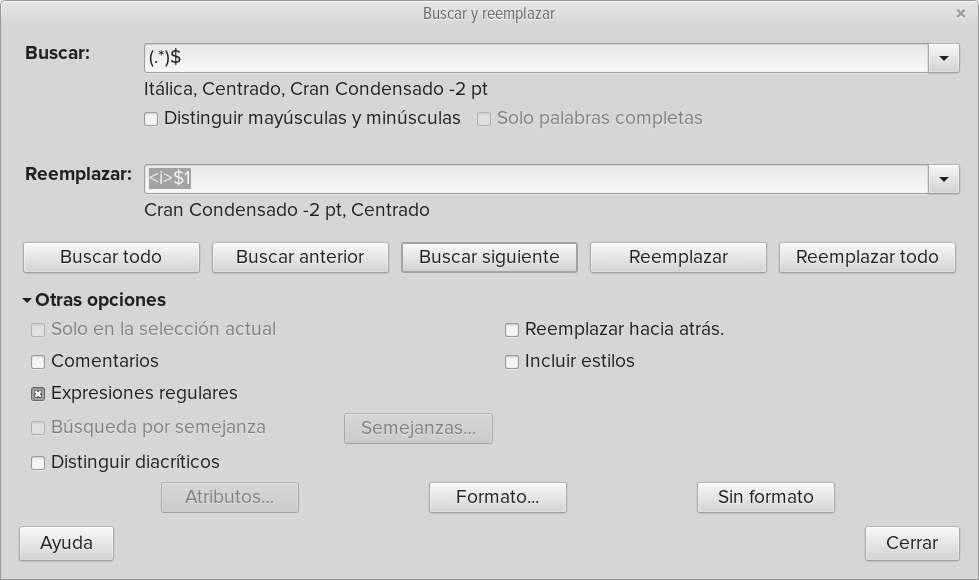
\includegraphics{images/searchandreplace.png}}
	\caption{Diálogo de búsqueda de LibreOffice.org.}
	\label{fig:searchandreplace}
\end{figure}	

Esta opción haría hipotéticamente posible salvar el texto en formato \ac{odt} y escribir un pequeño programa que llevara a cabo la preparación procesando el código \ac{xml} después de descomprimirlo. Al ser pocos los archivos en este formato, resulta más práctico tratarlos de forma manual. El inconveniente es que esto obliga a abordarlos de uno en uno, por lo que, de haber una cantidad grande de estos, convendría considerar procesar automáticamente el código \ac{xml}. De cualquier manera, conviene restringir las sustituciones desde el procesador de textos ofimático a aquellas que no puedan resolverse sencillamente en el archivo de texto con la línea de órdenes\index{línea de órdenes} del sistema operativo, ya que el tratamiento individual de los archivos acarrea un alto coste temporal.

\begin{figure}[!ht]
	\centering\small
	\resizebox{\linewidth}{!}{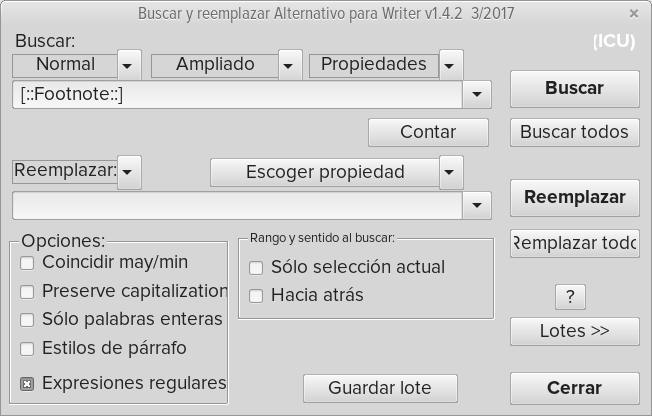
\includegraphics{images/asearchandreplace.png}}
	\caption{Extensión de búsqueda \emph{Alternative Find \& Replace for Writer}.}
	\label{fig:asearchandreplace}
\end{figure}

Para las sustituciones en el cuerpo del texto, se selecciona \texttt{Buscar y reemplazar}, que se encuentra en el menú \texttt{Editar}. Esto abre un diálogo con diferentes opciones para nuestro propósito (\Cref{fig:searchandreplace}). Aquí debe marcarse la casilla correspondiente para habilitar el uso de expresiones regulares\index{expresión regular}, y empezar a hacer las sustituciones requeridas. La expresión de la ilustración, por ejemplo, buscaría y capturaría (paréntesis) cualquier cadena de texto (\texttt{.*}) hasta el final de la línea ($\$$), siempre que la línea esté centrada y el texto en cursiva. Sustituiría el texto por el patrón capturado (todo hasta el final de la línea), pero, por ejemplo, con la cadena \texttt{<i>} antepuesta\footnote{La elección no es casual, sino que se aviene a las etiquetas del formato \ac{ved}, que veremos más en detalle algunas páginas más adelante.}, de modo que se identificaría esta línea una vez perdida la alineación y las propiedades del tipo de letra. Al pulsar \texttt{Reemplazar todo}, se aplicaría al texto completo. Sabemos también que los versos están alineados a la izquierda, mientras que el texto en prosa suele ir justificado a ambos lados de la página. Esto se aplica para buscar esta característica y marcar los pasajes necesarios.

Por su parte, para eliminar bloques paratextuales, también en el menú \texttt{Editar} seleccionaremos el elemento \texttt{Alt. buscar y reemplazer}\footnote{La errata está en el menú de la barra de tareas.}~[\textit{sic}]. Esto abre otro diálogo con opciones parecidas a la búsqueda estándar, aunque algo diferente (\Cref{fig:asearchandreplace}). Aquí también marcaremos la casilla que activa el uso de expresiones regulares\index{expresión regular}. En este caso, no buscaremos cadenas de texto, sino bloques (notas a pie de página, al final, etc.). Dejaremos vacío el campo con la sustitución, pues así indicaremos que el bloque buscado ha de reemplazarse por un elemento vacío. De esta manera, la expresión del ejemplo, eliminaría todo el cuerpo de notas a pie de página.

Los diferentes niveles de sangrado se indican mediante tabuladores, tantos como niveles haya. El espaciado interior también es de utilidad, ya que nos valdremos de él para diferenciar entre unidades estructurales. Una separación de un solo espacio divide componentes de una misma unidad, mientras que un número mayor de espacios vacíos indica una separación de otra índole. De esta manera, distinguiremos entre didascalia de personaje y parlamento con independencia de las propiedades del texto. El ejemplo \ref{ex:loctext} capturaría en un primer grupo la didascalia de personaje y en otro el parlamento, de manera que podríamos alterarlos de la manera más conveniente.

\begin{exe}
	\ex\label{ex:loctext}\texttt{\^{}\textbackslash s*(\textbackslash S+(?:\textbackslash s\textbackslash S+)*)(\textbackslash s\{2,\})(\textbackslash S+)\$}
\end{exe}

Podríamos modificar la expresión regular sustituyendo \texttt{\^{}\textbackslash s*}, que denota la presencia de cero o más (\texttt{*}) espacios (\texttt{\textbackslash s}), por un rango de entre $i$ y $j$ espacios, por ejemplo con \texttt{\^{}\textbackslash s\{$i$,$j$\}}, de manera que encontraríamos la presencia de versos compartidos. Así, adaptaríamos estas expresiones a los casos particulares y, de igual forma, abordaríamos el archivo de texto resultante.

\section{Escenario óptimo: XML-TEI}
El mejor caso posible es la conversión desde un archivo \ac{xmltei}. Este presenta todos los elementos necesarios para producir una forma estructurada y sin ambigüedades. El esquema de \Cref{fig:xmltei} muestra una descripción de la estructura básica de una obra de teatro, como las que se encuentran, por ejemplo, en DraCor. De la raíz \texttt{<TEI>} cuelgan dos ramas. La primera es \texttt{<TeiHeader>} es una cabecera de metadatos. La segunda es \texttt{<text>}, con el texto propiamente dicho, como se observa en el esquema de la jerarquía \ac{xmltei} (\Cref{fig:xmltei}). El estándar \ac{tei} define un detallado conjunto de etiquetas, cuyas directrices se extienden a lo largo de casi dos mil páginas en su última versión \parencite{tei2022}, por lo que aquí solo nos ocuparemos sucintamente de aquello que afecta directamente al análisis y, aun así, de manera muy superficial.
	
	\begin{figure}[!ht]
		\begin{forest}
			forked edges,
			%for tree={%
				%	edge path={\noexpand\path[\forestoption{edge}] (\forestOve{\forestove{@parent}}{name}.parent anchor) -- +(0,-12pt)-| (\forestove{name}.child anchor)\forestoption{edge label};}
				%}
			%forked edges,
			for tree={
				align=center,
				font=\tiny,
				%anchor = west,
				grow'=0, % tree direction
				%edge={->,>=latex},
				parent anchor=east, child anchor=west, % edge anchors
				%rounded corners, draw,
				text height=0.5ex, text depth=0.2ex % <<<<<<<<<<<<<
			}
			[\texttt{<TEI>}
			[\texttt{<teiHeader>}
			[\texttt{<fileDesc>}
			[\texttt{<titleStmt>}
			[\texttt{<title>}]
			[\texttt{<author>}]
			]
			[\texttt{<publicationStmt>}
			[\texttt{<authority>}]
			[\texttt{<publisher>}]
			[\texttt{<date>}]
			[\texttt{<availability>}
			[\texttt{<licence>}]
			]
			]
			[\texttt{<sourceDesc>}
			[\texttt{<bibl>}]
			[\texttt{<date>}]
			[\texttt{<idno>}]
			]
			]
			[\texttt{<particDesc>}
			[\texttt{<listPerson>}
			[\texttt{<person>}]
			[\texttt{<personGrp>}]
			[\texttt{...}]		
			]
			]
			[\texttt{<TextClass>}]
			]
			[\texttt{<text>}
			[\texttt{<front>}
			[\texttt{<castList>}
			[\texttt{<head>}]
			[\texttt{<castItem>}]
			[\texttt{...}]
			]
			]
			[\texttt{<body>}
			[\texttt{<div>}
			[\texttt{...>}
			[\texttt{<sp>}
			[\texttt{<speaker>}]
			[\texttt{<l>}]
			[\texttt{<stage>}]]
			[\texttt{...}]
			[\texttt{<stage>}]
			]
			[\texttt{...}]
			]
			[\texttt{...}]
			]
			]
			]
		\end{forest}
		\caption{Estructura de XML-TEI.}
		\label{fig:xmltei}
	\end{figure}

De la cabecera cuelgan otras subestructuras. En \texttt{<fileDesc>} hay información sobre la edición. Tal vez la más relevante de estas ramas sea \texttt{<titleStmt>}, pues incluye el título y el autor. Aquí se usan varias etiquetas, añadiendo argumentos si es necesario, como, por ejemplo, \texttt{<title type"main">} y \texttt{<title type"subtitle">}, para reflejar el título principal y el subtítulo, o crear una subsestructura en  \texttt{<author>} especificando detalles como nombre o apellidos. Los datos de la publicación cuelgan de \texttt{<publicationStmt>}, como la organización responsable de  la edición, en \texttt{<authority>}, la editorial en \texttt{<publisher>}, la fecha en \texttt{<date>} y la disponibilidad \texttt{<availibility>}, donde caben etiquetas como \texttt{<licence>} para expresar los términos legales de uso del texto (\ref{ex:publicationStmt}). Los datos de la obra original están bajo \texttt{<sourceDesc>}, con diversos identificadores, así como la fecha.

\begin{exe}
	\ex\label{ex:publicationStmt}\begin{lstlisting}[language=xml,upquote=true,numbers=none]
<publicationStmt>
    <authority>University of Vienna,Institute of Romance Languages and Literatures</authority>
    <publisher xml:id=""/>
    <date when="2022-01-12">
        <time when="14:08:57"/>
    </date>
    <idno type="quadramaX">La siembra del Señor (Los obreros del señor)</idno>
    <availability>
        <licence>
            <ab>CC-BY 4.0</ab>
            <ref target="https://creativecommons.org/licenses/by/4.0/">
                Licence
            </ref>
        </licence>
    </availability>
</publicationStmt>
\end{lstlisting}\end{exe}

Resulta de la mayor importancia la rama \texttt{<particDesc>}, ya que en ella se configura la lista de personajes que intervienen en la obra. Esta lista consta de una entrada única de tipo \texttt{<person>} para cada personaje\index{personaje} o, en el caso de personajes colectivos, de tipo \texttt{<personGrp>}, como ilustra el ejemplo \ref{ex:xmlid}. Asimismo, cada personaje se caracteriza más en detalle mediante atributos de la etiqueta, entre los cuales consideraremos dos. Tenemos, por ejemplo, \texttt{sex}, que se emplea para denotar si el personaje es masculino, femenino o lo que convenga. Otros atributos similares se emplean de manera análoga. Tanto o posiblemente más relevante para el tratamiento digital que los atributos de clase, es el identificador, pues asigna a cada uno de ellos un código individual que se mantiene a lo largo de la obra. Esto simplifica seguir a cada personaje, con independencia de que se referencia a un mismo locutor con diferentes didascalias, como abreviaturas, títulos de cortesía o, incluso, que un personaje cambie de nombre a mitad de la obra. Para ello, además de la didascalia bajo la etiqueta \texttt{<speaker>}, disponemos de un indicador paratextual \texttt{xml:id} único para cada personaje, siempre el mismo con independencia de la didascalia con que se nombre. De esta forma, una vez que hemos definido \texttt{xml:id="scipion"}, cada uno de los parlamentos del personaje llevará ese identificador, escríbase la didascalia \textsc{Scipión} o \textsc{Scip.}.  De esta manera, los versos bajo ambas se reconocen de forma sencilla como pertenecientes a un mismo personaje \textit{Scipión}.
\begin{exe}
\ex\label{ex:xmlid}\begin{lstlisting}[language=xml,upquote=true,numbers=none]
<person sex="MALE" xml:id="scipion">
    <persName>SCIPIÓN</persName>
</person>
<personGrp sex="UNKNOWN" xml:id="musicos">
    <persName>MÚSICOS</persName>
</personGrp>
\end{lstlisting}\end{exe}

Pueden existir más ramas de este árbol, algunas de las cuales resultan extremadamente útiles para facilitar la clasificación de la obra, como, por ejemplo, \texttt{<textClass>} (\ref{ex:textclass}). 

\begin{exe}
	\ex\label{ex:textclass}\begin{lstlisting}[language=xml,upquote=true,numbers=none]
<textClass>
	<keywords>
		</person>
		<term type="genreTitle">Comedia</term>
		<term type="subgenreTitle">De capa y espada</term>
	</keywords>
</textClass>
\end{lstlisting}\end{exe}

Respecto a los datos de la cabecera, cuantos más se encuentren a nuestra disposición, tantas más serán las posibilidades en lo concerniente al análisis del texto y en lo que atañe a cuestiones de archivo. Resulta evidente que la inclusión de la fecha inicial de la publicación, datos de los personajes\index{personaje} o del género de la obra permite cruzar esa información para buscar patrones. Pero no menos importantes son otras cuestiones, como la licencia de uso, que condicionará la manera de emplear los datos, o los identificadores de la obra y el autor, que facilitan la búsqueda y clasificación de esta. Las ediciones usadas proporcionan toda la información requerida, pero la cuestión podría cobrar importancia con fuentes menos minuciosas.

La rama \texttt{<text>} contiene el texto propiamente dicho, con dos partes denominadas \texttt{<front>} y \texttt{<body>}. Esta rama tiene la particularidad de que los contenidos de las etiquetas se muestran en el texto, por lo que los metadatos han de señalarse como atributos de la etiqueta. Bajo \texttt{<front>}, del ingleś \textit{front matter}, tendríamos, en principio, los preliminares. Sin embargo, en nuestro caso, aquí se incluye también el elenco bajo una estructura \texttt{<castList>} que contiene elementos del tipo \texttt{<castItem>} y \texttt{<head>}, este último para una cabecera del tipo «Personajes que hablan» o «\textit{Dramatis personae}».

La rama \texttt{<body>} se divide en partes bajo la etiqueta \texttt{<div>}. Aquí es habitual especificar el tipo y la numeración, cuando es necesario, para poder encontrar ramas bajo la etiqueta, como en \texttt{<div type="act" n="1">}. Bajo estas, puede haber asimismo subdivisiones, en la que, en lugar de \texttt{type="act"}, aparece, por ejemplo, \texttt{type="scene"} y, por lo general, especificando también la numeración. Finalmente, en la rama \texttt{<div>} más profunda, se encuentra el texto de la obra.

Este texto\footnote{Se trata de una codificación propia a partir de una edición todavía inédita de Ignacio Arellano del auto calderoniano \textit{La exaltación de la Cruz}.} tiene dos tipos principales de etiqueta, \texttt{<stage>} y \texttt{<sp>} (\ref{ex:parlamentos}). La primera señala las acotaciones\index{acotación} y la segunda los parlamentos. En estos últimos, además de la parte correspondiente al texto, debe tenerse muy en cuenta el atributo  \texttt{who} de la etiqueta, que es el identificador único que se había definido en la cabecera y que permite, por ejemplo, encontrar redes de relaciones entre personajes\index{personaje}. Es preferible usar este identificador en lugar de la etiqueta \texttt{<SPEAKER>}, ya que esta se refiere a la didascalia y no al locutor, por lo que, como indicamos, pude variar, lo que dificultaría su seguimiento. La última etiqueta que nos interesa es \texttt{<l>}, que marca cada línea.

Además del atributo \texttt{n} que, como los elementos anteriores, denota la numeración, puede aparecer el atributo \texttt{part}. Este sirve para indicar el comienzo de un verso (\texttt{"I"}), su continuación (\texttt{"M"}) y su término (\texttt{"F"}), para identificar versos distribuidos a lo largo de dos o más líneas. Podría darse el caso de que, en lugar de la etiqueta \texttt{<l>}, halláramos otra del tipo \texttt{<p>}. Esta denotaría que no encierra una línea de parlamento, sino un párrafo y, por lo tanto, prosa. Se emplea, por ejemplo, cuando un personaje lee una carta. Tampoco es raro que, inmediatamente bajo \texttt{<sp>}, no se abra un bloque mediante una etiquetas de tipo \texttt{<l>}, sino que sea una estructura intermedia \texttt{<lg>} y, por debajo de esta, se encontrarían las líneas. Por ejemplo, \texttt{<lg type="stanza">}. Las acotaciones internas se representan mediante etiquetas \texttt{<stage>} dentro de una estructura \texttt{<sp>}, en lugar de a su mismo nivel como las externas.


\begin{exe}
	\ex\label{ex:parlamentos}\begin{lstlisting}[language=xml,upquote=true,numbers=none]
<sp who="#morlaco">
    <speaker>MORLACO</speaker>
    <l met= "+-++-++--+-" rhyme="ina">¿Yo beldad? Loco me es sobre gallina</l>
    <l part="I">este príncipe.</l>
</sp>
<sp who="#siroes">
    <speaker>SIROES</speaker>
    <l part="M">¿Dónde...</l>
</sp>
<sp who="#morlaco">
    <speaker>MORLACO</speaker>
    <l part="F" met="+-+--+-+++-" rhyme="ada">No sé nada</l>
    <l n="1665" met="+--+++-+-+-" rhyme="ada">y hágase allá, que es burla muy pesada.</l>
</sp>
\end{lstlisting}\end{exe}

Cabe la posibilidad de incluir atributos \texttt{met} para el patrón rítmico y \texttt{rhyme} para la rima. No resulta común encontrarlo en textos españoles y, de hecho, no hemos hallado ninguna edición que lo incluya, aunque sea bastante habitual en lenguas clásicas, el griego sobre todo. Así que, si de bien poco sirve tener la posibilidad en el análisis careciendo de textos que hagan uso de ella, la recordaremos para aprovecharla más adelante y reflejar los resultados de nuestros análisis.

Conociendo la estructura, la extracción de datos resulta trivial: recorremos recursivamente las subestructuras de \ac{xmltei}  hasta llegar al nivel más profundo de cada rama, leemos los datos que en ella se encuentran y los tratamos de la manera que resulte más conveniente. Por ejemplo, para tratar los parlamentos procederemos como en \Cref{list:xml2txt}.

\begin{algorithm}[!ht] %or another one check
	\caption{Conversión de XML-TEI a texto.}\label{list:xml2txt}
%	\Ffuncion{\Reordena{tei2txt}}{
%		\cuerpo \gets\ \texttt{<body>} \;
%		\actos \gets\ cuerpo.encuentra(\texttt{<div>}) \;
		\ForEach{$acto \in\:actos$}{
			\ForEach{$escena \in\:acto$}{
				\ForEach{$estructura \in\:escena$}{
					\If{$estructura\: \is\: parlamento$}{
						\ForEach{$l\acute{\imath}nea \in\:estructura$}{
							\If{$(\neg\:part\:\vee part = \langle F\rangle)$}{
								\guardaverso{$anteriores + l\acute{\imath}nea$} \;
								anteriores \gets $\emptyset$
							}
							\Else{anteriores \gets $anteriores + l\acute{\imath}nea$}
						}
					}
					\Else{\guardaac{estructura}}
				}
			}
		}
\end{algorithm}

El algoritmo consiste en recorrer los actos, y en cada uno de ellos —supondremos que no hay escenas ni otros niveles intermedios—, recorremos a su vez las estructuras inferiores, como los parlamentos y acotaciones. Aquí se bifurca el flujo de datos según el tipo de estructura. Si es un parlamento, lo recorremos línea a línea. Primero probamos si la línea se corresponde a un verso, comprobando que la línea no lleva atributo de parte o es la sección terminal de un verso. En este caso, procesaremos las partes anteriores del verso —que será un elemento nulo de no ser un verso compartido—, seguidas de esta línea y reiniciamos la variable intermedia donde guardamos los elementos anteriores. Si la línea no es terminal, vamos añadiendo las nuevas partes del verso a la variable intermedia. Si, por el contrario, la estructura no es un parlamento, la procesaremos como acotación\index{acotación}. De manera análoga, haremos lo propio con todos los elementos de la cabecera, aunque, en ese caso, los terminales serán normalmente de un solo tipo —con excepciones como la descripción de los personajes\index{personaje}— y no hará falta recorrer en un bucle, sino buscar determinados elementos únicos.

\section{Precauciones con la codificación}
Hasta aquí hemos visto las estructuras de datos como meras abstracciones. Sin embargo, a la hora de trabajar en la práctica con ellas, debemos observar ciertas precauciones de índole más técnica que conceptual, ya que estamos sujetos a la representación interna de los caracteres del texto empleada por el computador. Incluso cuando el procedimiento empleado por todos los archivos de texto es muy similar, hay algunas diferencias en la codificación que son susceptibles de causar dificultades y errores. En nuestro trabajo, esto redunda tanto en la organización de los textos como en la manera de tratar las fuentes. Para entender el problema nos remontaremos a los primeros estándares de codificación informática de texto.

En las computadoras personales típicas, el máximo común divisor es  \textit{American Standard Code for Information Interchange} básico, más conocido por sus siglas \ac{ascii} \parencite{wells1997}. Este estándar surgió a principios de la década de 1960 a expensas de la American Standard Association. Se diseñó con el objetivo de representar textos escritos en inglés y, más específicamente, de la variedad americana de esta lengua. Por este motivo, no era capaz de mostrar caracteres ajenos a ese alfabeto, como los que emplean muchas lenguas europeas, el español entre ellas. La cantidad de caracteres no alfanuméricos también estaba limitada y, por ejemplo, no preveía el uso de símbolos monetarios distintos del dólar estadounidense. Como es de suponer, otros sistemas de escrituras no basados en el alfabeto latino quedaban totalmente excluidos. Este \ac{ascii} se representa mediante 7 bits, por lo que hay un máximo de $2^7$ combinaciones, que se reparten entre 95 \textit{caracteres}\index{carácter} imprimibles\index{carácter!imprimible} y 33 de control\index{carácter!de control}\footnote{Un carácter no equivale necesariamente a un grafema\index{grafema}, sino a un patrón de bits al que le corresponde un significado. Este admite diferentes formas: puede ser gráfico —una letra, un signo, un símbolo o un espacio en blanco—, en cuyo caso hablaremos de caracteres imprimibles, pero también puede representar una acción no visible —borrar el carácter anterior o marcar el final de una línea—, y hablaremos de caracteres de control \parencite[139]{haralambous2019}.} en su revisión más moderna \parencite[423-433]{mackenzie1980}. 

Esta codificación es precisamente la que usa el \textit{Speech Assessment Methods Phonetic Alphabet} (\ac{sampa}). Se trata de un alfabeto que se desarrolló en el marco del proyecto European Strategic Programme on Research in Information Technology (\ac{esprit}) de la Comunidad Económica Europea para representar en soporte informático la fonología de lenguas europeas occidentales. Una de las premisas de su diseño era que debía garantizar la compatibilidad con las computadoras de la época. De acuerdo con esto, podríamos valernos de ella para representar las transcripciones fonológicas. Sin embargo, esto presentaría problemas para los fragmentos grafémicos.

Debido a las limitaciones de \ac{ascii}, diversos fabricantes y organizaciones concibieron sus propios métodos de codificar los caracteres extendidos, entre los que se encuentran las letras con diacrítico y muchos de los signos de puntuación que necesitamos para escribir en español. Así, encontramos que la \ac{iso} propuso su estándar ISO-8859-1 y Microsoft desarrolló Windows-1252 para las lenguas europeas. Ambos son de 1 byte, lo que son suficientes para representar $2^8$ combinaciones o, lo que es lo mismo, 256 caracteres.

Hoy en día, hemos superado aquellas constricciones impuestas por la técnica, podemos representar en texto plano no solo todas las grafías que demanda una correcta ortotipografía en cualquier lengua europea, sino muchos más caracteres. El desarrollo de las computadoras personales hizo irrelevantes las limitaciones que prevenían la aparición de nuevos sistemas de codificación. \textit{Unicode}\index{Unicode} se presentó en 1991 con la idea de ofrecer una solución a las constricciones de las  codificaciones existentes y, especialmente, para dar soporte a todas las lenguas vivas y muertas, así como otros sistemas de símbolos cuya inclusión estuviera justificada. Cada carácter Unicode tiene el mismo número de bits, por lo que todos ellos se codifican como un único carácter para cada grafema, tanto del español como del \ac{afi}. Por defecto, Unicode emplea dos bytes para representar un solo carácter, esto es, dieciséis bits. Esto permite usar un total de $2^{16}$ o, lo que es lo mismo, 65{.}536 caracteres \parencite{bettels1993}. Los sistemas operativos modernos de tipo Unix\index{Unix} más extendidos —Linux\index{Linux} y MacOS\index{MacOS}— soportan Unicode\index{Unicode} de forma nativa en prácticamente todas sus versiones posteriores al año 2000. De esta manera, no resulta ya necesario emplear \ac{sampa}, pues pueden representarse con la misma codificación tanto los textos grafémicos españoles como su transcripción al \ac{afi}.

Esto no solo simplifica la comprensión del texto, ya que la notación de los programas se corresponde con la impresa, sino que tiene implicaciones en el análisis informático de los textos transcritos. En concreto, la limitación del número de caracteres disponibles obliga a que SAMPA represente dígrafos y ligaturas mediante dos caracteres, mientras que Unicode los representa con uno. Por ejemplo, SAMPA obligaría a preprocesar el fonema /\texttoptiebar{tʃ}/ al representarlo con los caracteres ASCII \textit{t} y \textit{S}, como \textit{tS}. Unicode, por su parte, aúna los símbolos del \ac{afi} \textit{t} y \textit{ʃ} mediante un único carácter digrafémico \textsc{\textit{ʧ}}. De esta manera, se vuelve innecesario crear una excepción para tratar este sonido africado\index{consonante!africada}, al poder representarse como una única unidad.

Aunque el formato final de nuestros datos está codificado según Unicode\index{Unicode}, esto no implica necesariamente que los archivos de origen también opten por el mismo sistema. Por lo tanto, hay que convertir aquellos archivos de texto que partan de codificaciones distintas. En el caso de \ac{ascii}, no sería necesario porque es un subconjunto de Unicode\index{Unicode}; desafortunadamente, como ya dijimos, es un subconjunto que no incluye todos los diacríticos y signos ortográficos necesarios para escribir en español de acuerdo con su ortografía, por lo que ningún texto aceptado va a estar en \ac{ascii} puro. Las otras aproximaciones de un byte a la representación de caracteres extendidos provocan serios problemas, pues producen artefactos que alteran el texto (\Cref{fig:codificacion}). Si bien los signos ortográficos no afectarían a nuestro propósito, los diacríticos supondrían un problema grave. Por lo tanto, se hace necesario unificar formatos en algún momento y, por razones prácticas, lo haremos cuanto antes. 

\begin{figure}[!ht]
	\centering
	\footnotesize
	\begin{subfigure}{.5\textwidth}
		\texttt{¡Oíd, mortales, oíd,\\
			y al pregón de la Fama\\
			todos acudid!}
	\end{subfigure}%
	\begin{subfigure}{.40\textwidth}
		\texttt{¡Oà d, mortales, oà d,\\
			y al pregón de la Fama\\
			todos acudid!}
	\end{subfigure}
	\caption{Transliteración de la variante ASCII ISO-8859-15 a Unicode.}
	\label{fig:codificacion}
	\normalsize
\end{figure}

La solución pasa por identificar de antemano el tipo de codificación y convertir el archivo a Unicode\index{Unicode}. Esto no presenta mayor problema en un entorno Unix\index{Unix}, cuyas herramientas proveen soluciones simples. Mediante el mandato \texttt{file} identificamos la codificación del archivo y, utilizando un programa al efecto\footnote{Por poner dos ejemplos de entre los empleados, la biblioteca \ac{gnu} C de Linux\index{Linux} provee \texttt{iconv} y MacOS\index{MacOS} dispone de \texttt{textutil} para la tarea.}, solventamos el inconveniente.

 A pesar de que Unicode es la opción que mejor se adapta a nuestro propósito, tampoco está exenta por completo de algunas fuentes potenciales de complicaciones. Una de ellas, que debemos señalar para poder evitarla, deriva del propio diseño de la codificación.  Aunque esta se adecúa a las ortografías de las lenguas más conocidas y es capaz de representar un gran número de caracteres, soluciona las combinaciones de dos maneras diferentes, indistinguibles para el ojo, pero no precisamente triviales de tratar digitalmente de manera elegante. Para representar un carácter compuesto, pongamos por ejemplo la letra eñe minúscula, se usa la codificación Unicode\index{Unicode} simple \textsc{latin small letter n with tilde}. Esta es el carácter U+00F1 para el computador y, para nosotros, el grafema \textlangle{}ñ\textrangle. También existe la posibilidad de representarlo mediante la combinación de los caracteres \textsc{latin small letter n} \textlangle{}n\textrangle{} y \textsc{combining tilde} \textlangle$\tilde{\text{\DVS◌}}$\textrangle. En este último caso, aunque nosotros veríamos igualmente el grafema \textlangle{}ñ\textrangle{} en la pantalla, el computador leería la secuencia U+006E U+0303: esto es, dos caracteres. Como dijimos, hasta aquí no sería problema para atenerse a la ortografía española. Desafortunadamente, no puede decirse lo mismo de otros sistemas de representación. 

Concretamente, las vocales no silábicas, marcadas con un símbolo diacrítico de breve invertida inferior \textlangle\textsubarch{{\DVS◌}}\textrangle, solo admiten representación en Unicode mediante una combinación, de forma que hemos de tratarlo como dos caracteres \parencite[17]{moran2018}. Por esta razón, ante la dicotomía de introducir excepciones en el código por una cuestión técnica visual o mantener la fidelidad a los principios rectores, optamos por lo segundo, dando primacía a la claridad conceptual del proceso sobre la estética del resultado\footnote{Dejamos abierto para  futuras versiones de la biblioteca modificar esto.}. De este modo, representaremos las semivocales /\textsubarch{i}/ y /\textsubarch{u}/ con el mismo símbolo que las semiconsonantes /j/ y /w/, respectivamente\index{semivocal}\index{semiconsonante}\index{vocoide}, y usaremos el carácter individual con diacrítico de breve integrado (\textlangle{ă}\textrangle, \textlangle{ĕ}\textrangle{} y \textlangle{ŏ}\textrangle) para el resto de vocoides.

La codificación de los símbolos que señalan acentos primarios o secundarios en las sílabas  (ˈ, ˌ) no se ven afectados gracias a que, al contrario que los modificadores diacríticos, estos anteceden a la sílaba que modifican. Por consiguiente, cuando aparece uno, se tiene en cuenta como modificador, pero se ignora para lo demás \textit{a priori}.

Otro problema que se plantea son las distintas formas en las que los diferentes sistemas representan el final de línea (\textsc{lf}) y el retorno de carro  (\textsc{cr}). Las máquinas con un sistema operativo de tipo Unix\index{Unix} —GNU/Linux\index{Linux} y MacOS\index{MacOS}, por ejemplo—, emplean únicamente \textsc{lf}. Por su parte, los computadores Windows\index{Windows} usan \textsc{cr} \textsc{lf}, mientras que sistemas Apple antiguos emplean \textsc{cr}. Esto supone para nosotros que, cuando abrimos un texto con saltos de línea para Windows, veremos al final de cada fila un artefacto correspondiente al carácter \textsc{cr}, sin uso en nuestro sistema. En un texto creado en una máquina Apple antigua, lo que aparecerá será tan solo una larga línea con artefactos dispuestos a intervalos, ya que no tenemos el carácter \textsc{lf} que indica el final de la línea, pero sí \textsc{cr}, para el que no encontramos uso.  Por esta razón, es necesario convertir aquellos textos que así lo requieran. De nuevo, usaremos la herramienta estándar de Unix \texttt{file} para identificar el tipo de final de línea que tenemos y programas específicos para convertir las marcas de un sistema a otro\footnote{Bajo Linux\index{Linux}, \texttt{mac2unix} o \texttt{dos2unix} o \texttt{textutil} en MacOS\index{MacOS}. Se puede hacer usando tan solo las herramientas estándar de Unix\index{Unix}, como \texttt{sed} o \texttt{awk}.}.

Una vez podemos manipular las fuentes para tratar el texto con la asistencia del computador, nos hallamos en condiciones de empezar a identificar y clasificar las entidades que requerimos para caracterizar la obra teatral. En realidad, como veremos en el capítulo siguiente, la cuestión no es tanto encontrar estos elementos, pues ya hemos visto que la codificación \ac{xmltei} ha resuelto este reto y proporciona un buen modelo, sino seleccionar aquellos componentes que necesitemos, así como encontrar una disposición que facilite los análisis cuantitativos. 
